\section*{Lucrarea de laborator \#4}
\phantomsection

\section{Obiectivele lucrarii}
Cunostinte de baza privina arhitectura unei aplicatii mobile
~\\
Cunostinte de baza ale platformei SDK

\section{Scopul lucrarii de laborator}
Realizarea aplicatiei TIC-TAC-TOE pe \textbf{IOS}
~\\
Regim de joc Player vs Player.
~\\
Regim de joc Player vs AI (Artificial Intelligence).

\section{Mersul lucrarii de laborator}

\tab Drept IDE am folosit XCode. Ca limbaj de programare a fost folosit
\textbf{Objective-C}. Aplicatia data nu este Cross-Platform. Aplicatiile
nativ au un avantaj ca lucreaza mai rapid.Aplicatia este single-view. Deci va fi doar un singur view.
El are urmatoarea structura.
~\\
\begin{center} 
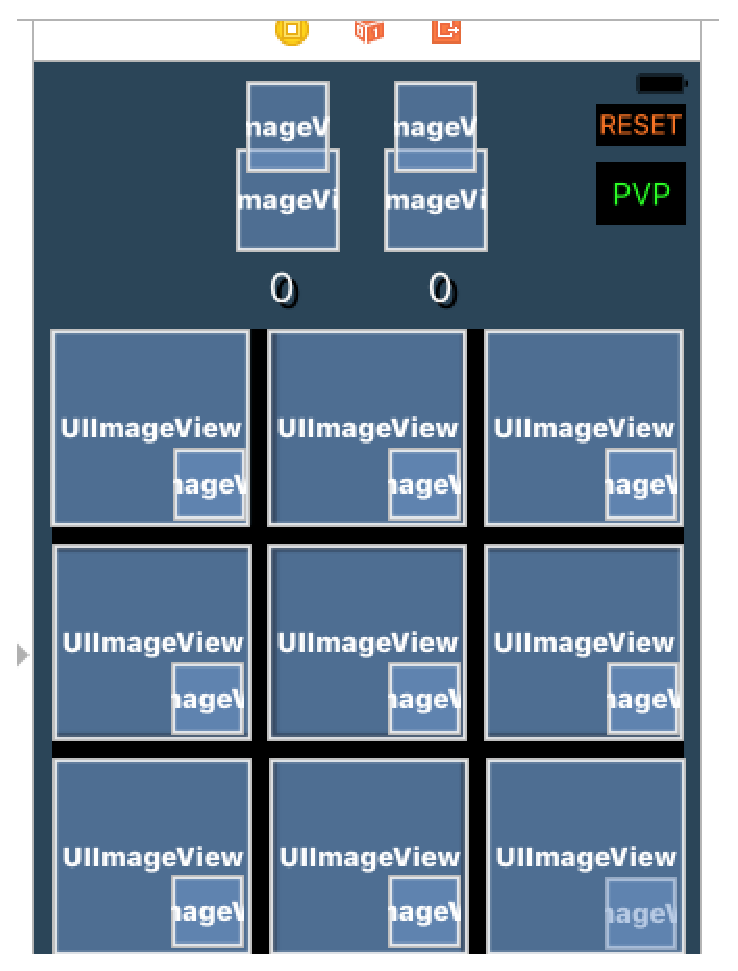
\includegraphics[width=7cm, height=7.5cm]{1.eps}
\end{center}
\clearpage

\tab \textbf{Screenshoturi din procesul crearii}
\begin{center} 
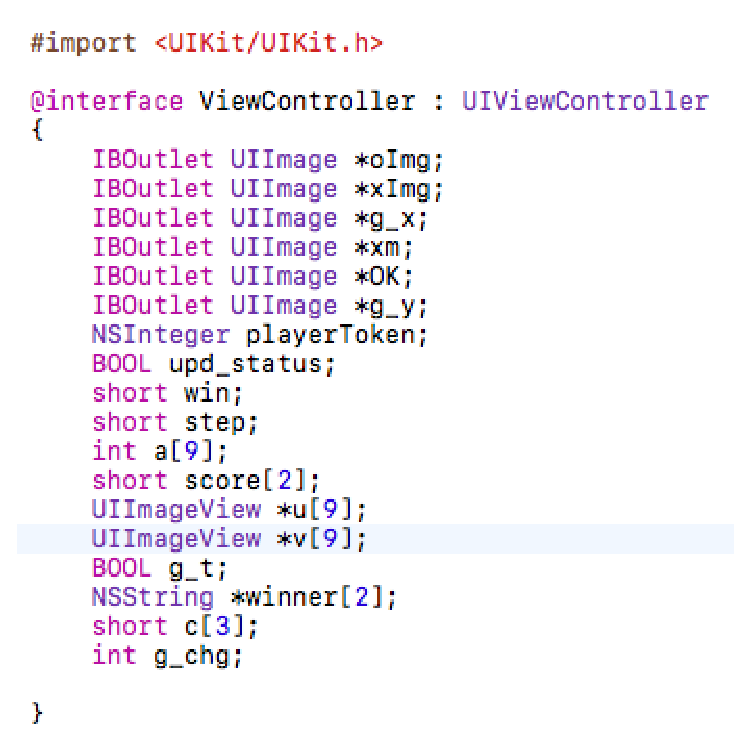
\includegraphics[width=9cm, height=7.5cm]{2.eps}
\end{center}
\begin{center} 
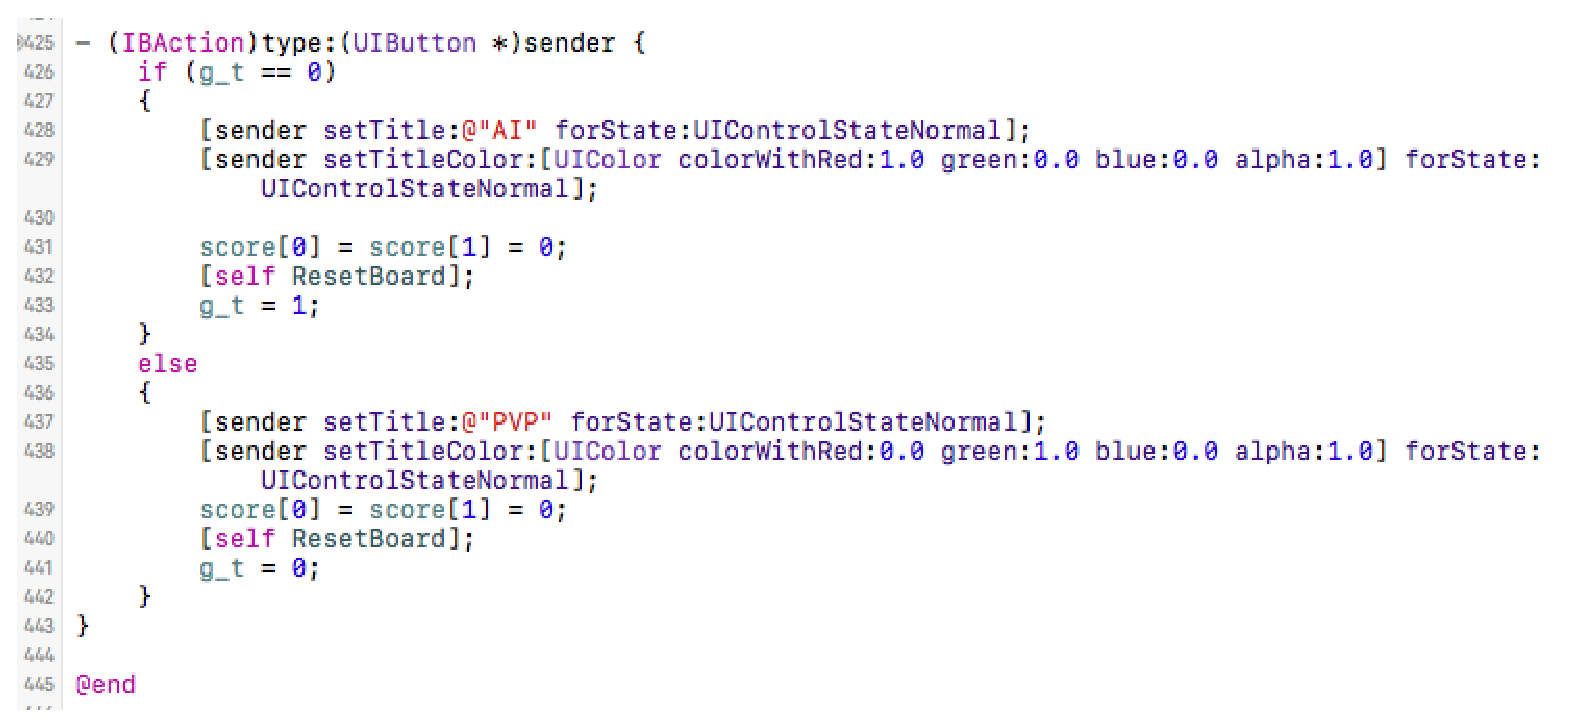
\includegraphics[width=13cm, height=6.5cm]{3.eps}
\end{center}

\clearpage
\section{App Screenshots}
\textbf{Game process}
\begin{center} 
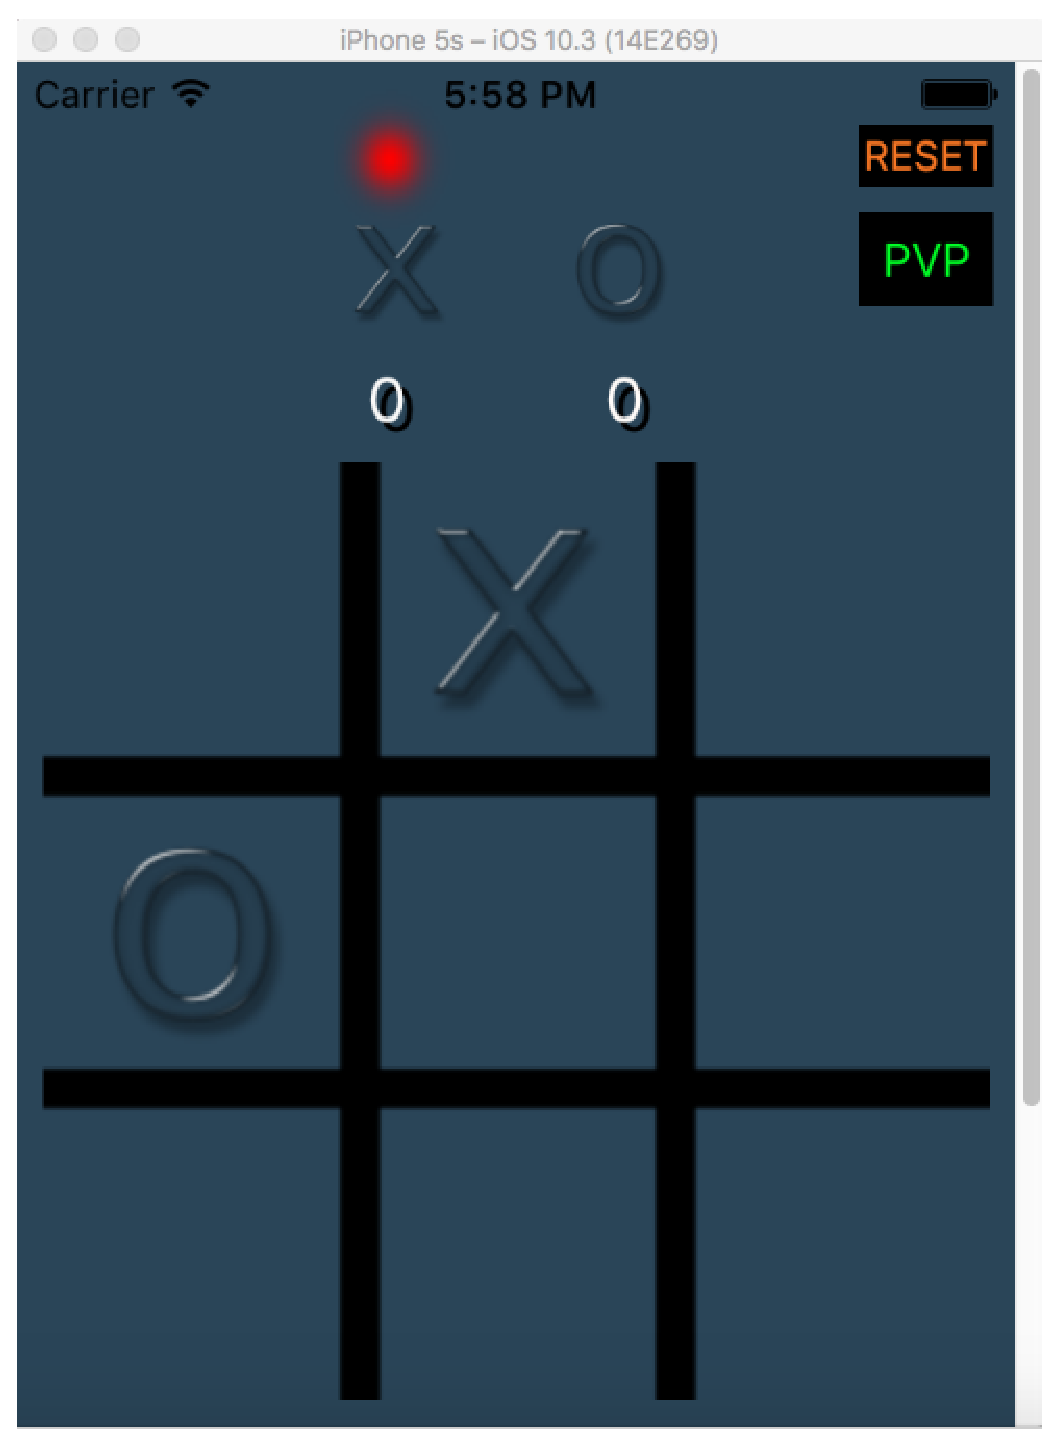
\includegraphics[width=7cm, height=8.5cm]{4.eps}
\end{center}
\begin{center} 
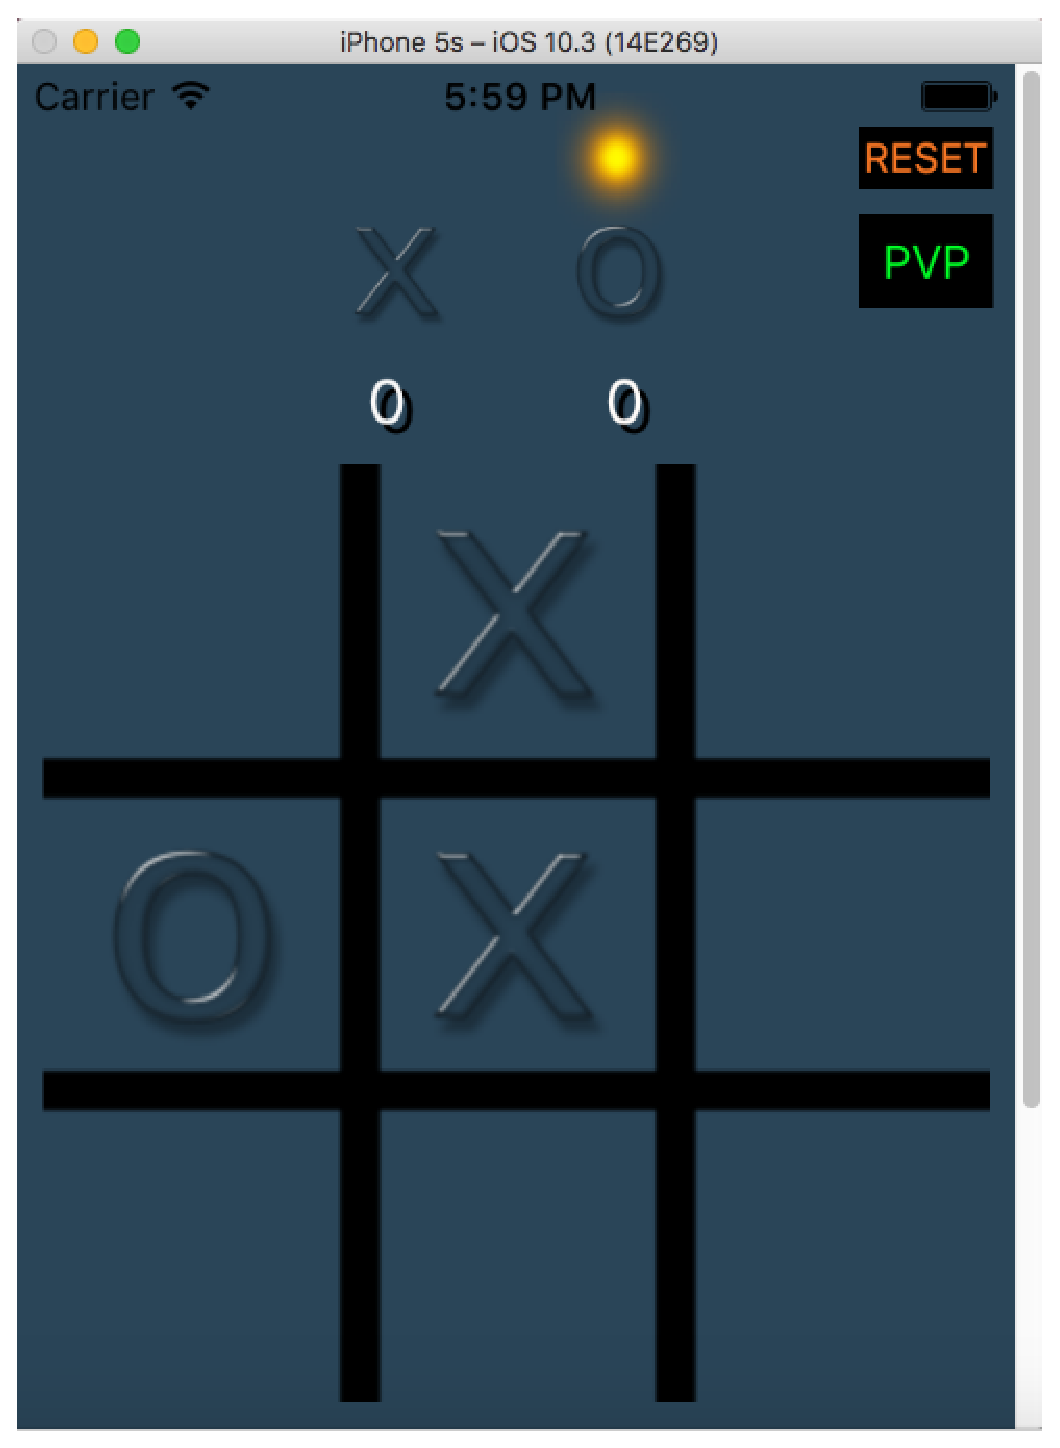
\includegraphics[width=7cm, height=8.5cm]{5.eps}
\end{center}
\textbf{Winner}
\begin{center} 
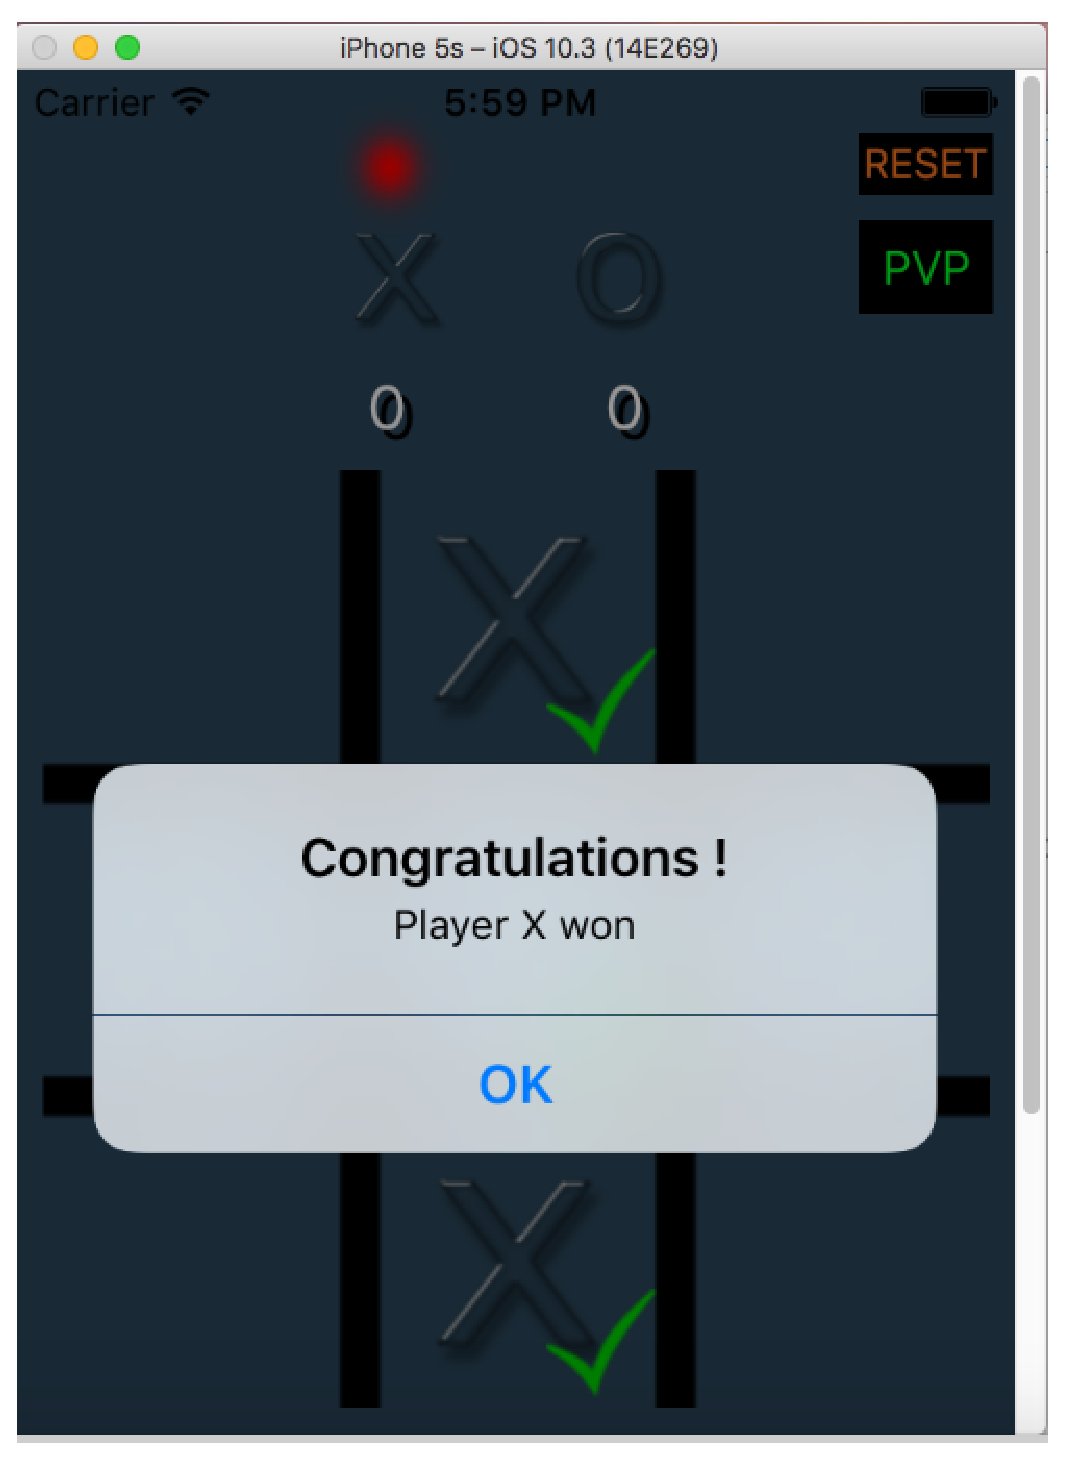
\includegraphics[width=7cm, height=9cm]{6.eps}
\end{center}
\begin{center} 
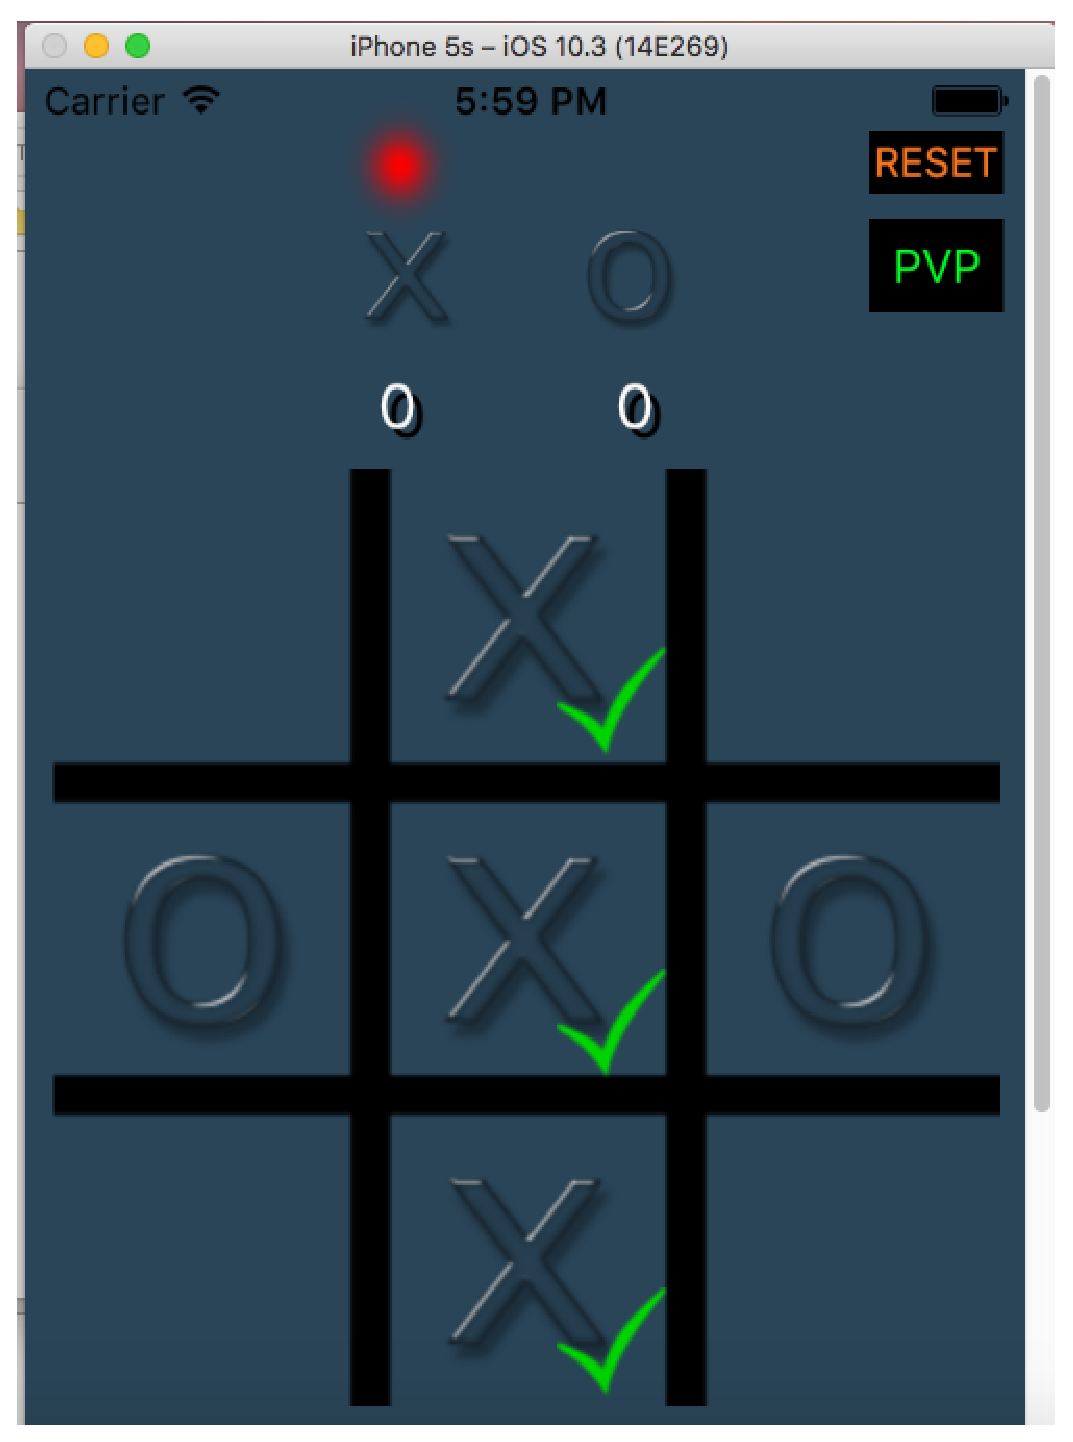
\includegraphics[width=7cm, height=9cm]{7.eps}
\end{center}
\textbf{No Winner}
\begin{center} 
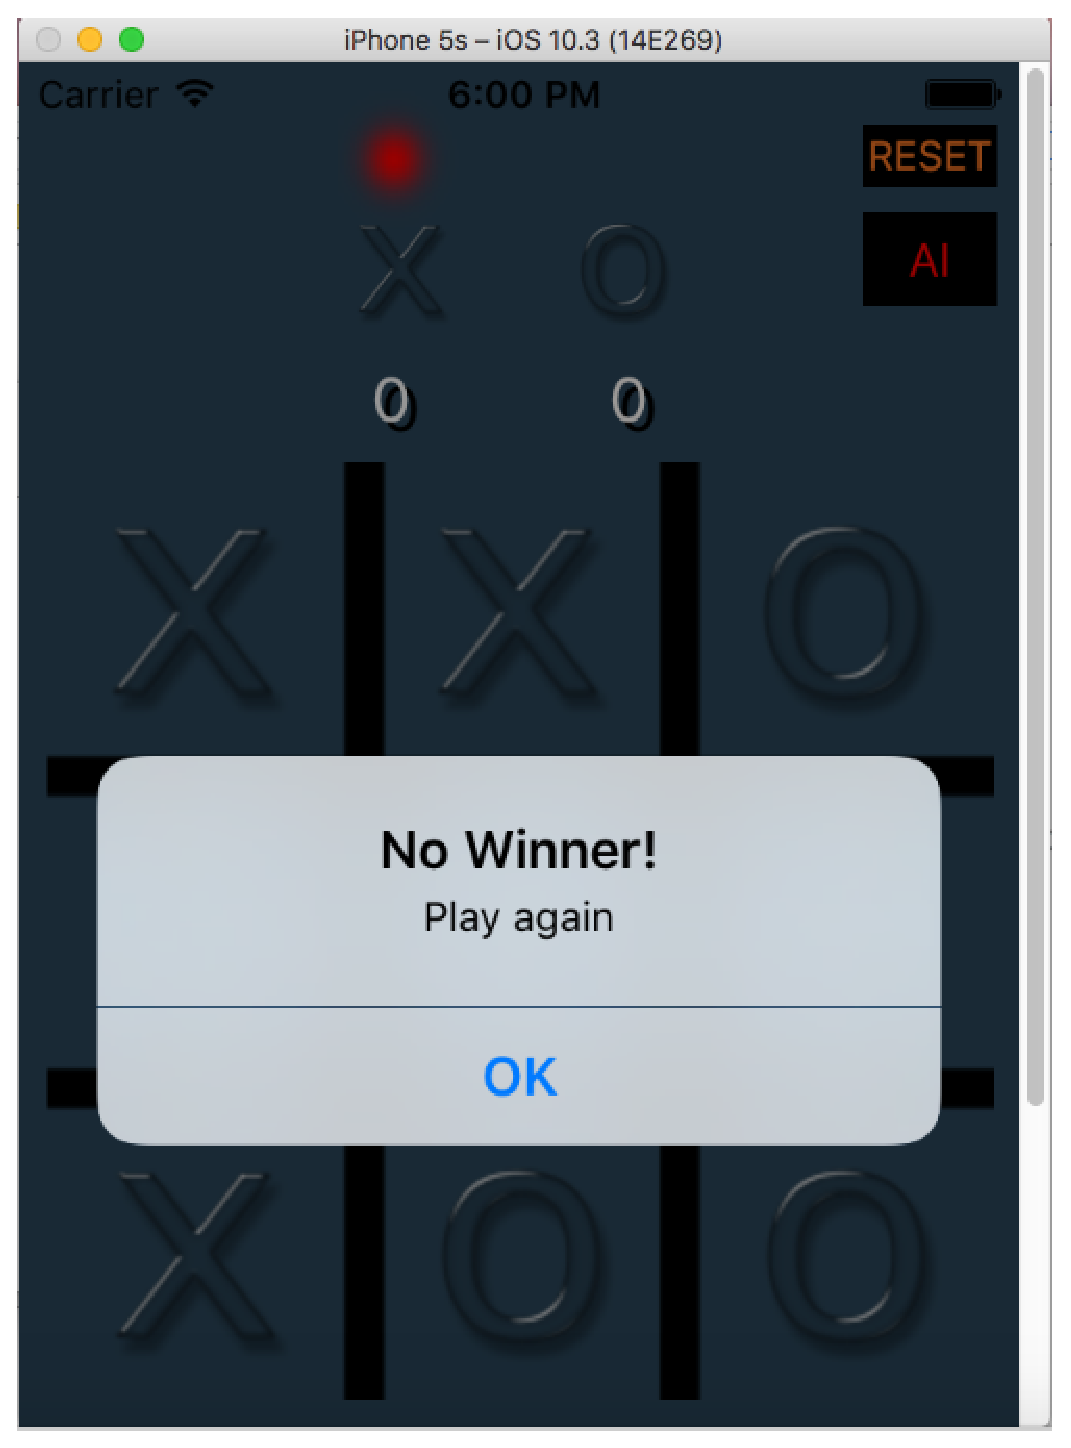
\includegraphics[width=7cm, height=9.5cm]{8.eps}
\end{center}
\clearpage

